\begin{figure}[H]
    \centering
    \caption{MRU cache given: A,B,C,D,B,D,A}
    \label{fig:my_label}
\begin{tikzpicture}
\node[rounded corners,draw=black,label=above:MRU, minimum size=2cm] (a) at (0,0)  {
    \begin{tikzpicture}
        \node[rounded corners,draw=black,minimum size=0.8cm]{A};
    \end{tikzpicture}
    
\begin{tikzpicture}
        \node[rounded corners,draw=black,minimum size=0.8cm]{};
    \end{tikzpicture}
    
\begin{tikzpicture}
        \node[rounded corners,draw=black,minimum size=0.8cm]{};
    \end{tikzpicture}
    };
    \node[text width=3cm] at (-3, 0) 
    {Miss on A as first instance, add A to cache};

    
    \node[rounded corners,draw=black,minimum size=2cm] (b) at (0,-2.5)  {   
\begin{tikzpicture}
        \node[rounded corners,draw=black,minimum size=0.8cm]{A};
    \end{tikzpicture}
    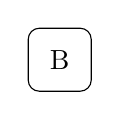
\begin{tikzpicture}
        \node[rounded corners,draw=black,minimum size=0.8cm]{B};
    \end{tikzpicture}
    
\begin{tikzpicture}
        \node[rounded corners,draw=black,minimum size=0.8cm]{};
    \end{tikzpicture}
    };
     \node[text width=3cm] at (-3,-2.5) 
    {Miss on B as first instance, add B to cache};
    
    \node[rounded corners,draw=black,minimum size=2cm] (c) at (0,-5)  {   
\begin{tikzpicture}
        \node[rounded corners,draw=black,minimum size=0.8cm]{A};
    \end{tikzpicture}
    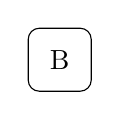
\begin{tikzpicture}
        \node[rounded corners,draw=black,minimum size=0.8cm]{B};
    \end{tikzpicture}
    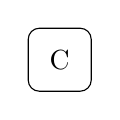
\begin{tikzpicture}
        \node[rounded corners,draw=black,minimum size=0.8cm]{C};
    \end{tikzpicture}
    };

    \node[text width=3cm] at (-3,-5) 
    {Miss on C as first instance, C added to cache};
      
    \node[rounded corners,draw=black,minimum size=2cm] (d) at (0,-7.5)  {   
\begin{tikzpicture}
        \node[rounded corners,draw=black,minimum size=0.8cm]{A};
    \end{tikzpicture}
    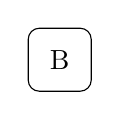
\begin{tikzpicture}
        \node[rounded corners,draw=black,minimum size=0.8cm]{B};
    \end{tikzpicture}
    
\begin{tikzpicture}
        \node[rounded corners,draw=black,minimum size=0.8cm]{D};
    \end{tikzpicture}
    };

     \node[text width=3cm] at (-3,-7.5) 
    {Miss on D as first instance, evict C since MRU};
    
    \node[rounded corners,draw=black,minimum size=2cm, below left=1 cm of d] (e) at (2.2,-8.4)  { 
    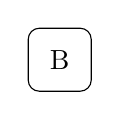
\begin{tikzpicture}
        \node[rounded corners,draw=black,minimum size=0.8cm]{B};
    \end{tikzpicture}
    
\begin{tikzpicture}
        \node[rounded corners,draw=black,minimum size=0.8cm]{D};
    \end{tikzpicture}
    
\begin{tikzpicture}
        \node[rounded corners,draw=black,minimum size=0.8cm]{A};
    \end{tikzpicture}
    };  

     \node[text width=3cm] at (-3,-10) 
    {Hit on B};

    \node[rounded corners,draw=black,minimum size=2cm, below left=1 cm of d] (f) at (2.2,-11)  { 
    
\begin{tikzpicture}
        \node[rounded corners,draw=black,minimum size=0.8cm]{A};
    \end{tikzpicture}
    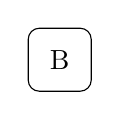
\begin{tikzpicture}
        \node[rounded corners,draw=black,minimum size=0.8cm]{B};
    \end{tikzpicture}
    
\begin{tikzpicture}
        \node[rounded corners,draw=black,minimum size=0.8cm]{D};
    \end{tikzpicture}
    };  

     \node[text width=3cm] at (-3,-12.5) 
    {Hit on D};

    \node[rounded corners,draw=black,minimum size=2cm, below left=1 cm of d] (g) at (2.2,-13.5)  { 
    
\begin{tikzpicture}
        \node[rounded corners,draw=black,minimum size=0.8cm]{A};
    \end{tikzpicture}
    
\begin{tikzpicture}
        \node[rounded corners,draw=black,minimum size=0.8cm]{D};
    \end{tikzpicture}
    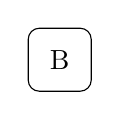
\begin{tikzpicture}
        \node[rounded corners,draw=black,minimum size=0.8cm]{B};
    \end{tikzpicture}
    };  

     \node[text width=3cm] at (-3,-15) 
    {Hit on A};

    \draw[thick,->] (a) -- (b);
    \draw[thick,->](b) -- (c);  
    \draw[thick,->](c) -- (d);  
    \draw[thick,->](d) -- (e);  
    \draw[thick,->](e) -- (f);  
    \draw[thick,->](f) -- (g);  
\end{tikzpicture}
\end{figure}